\subsection{Generación de señalamiento paso a paso}

	Al ejecutar el RNA, primero detectará todos los \textit{netElements}, sus coordenadas iniciales y finales en la topología, y el sentido en el que fueron definidas. El resultado obtenido se muestra en el Cóodigo \ref{lst:EJ6_1}.
	
	\begin{lstlisting}[language = {}, caption = Detección de \textit{netElements} por parte del RNA , label = {lst:EJ6_1}]
	###### Starting Railway Network Analyzer #####
	Reading .railML file
	Creating railML object
	Analyzing railML object
	Analyzing graph
	ne1 [-1500, 450] [-600, 450] >>
	ne2 [-600, 450] [-300, 750] >> 
	ne3 [-600, 450] [300, 450] >>
	ne4 [300, 450] [1350, 750] >>
	ne5 [300, 450] [1200, 450] >>
	ne6 [-300, 750] [480, 750] >>
	ne7 [-300, 750] [1530, 1020] >>
	ne10 [1200, 450] [1950, 750] >>
	ne11 [1200, 450] [1950, 450] >>
	ne41 [1530, 1020] [2790, 1320] >>
	ne42 [1530, 1020] [390, 1260] <<
	The network is connected
	\end{lstlisting}
	
	Por ejemplo, el \textit{netElement} ne42 inicia en la coordenada (1530;1020) y finaliza en la coordenada (390;1260). El símbolo $<<$ indica que ne42 se encuentra definido de derecha a izquierda, ya que la componente x de la coordenada final es mayor a la de la coordenada inicial. En este caso la componente y es diferente en ambas coordenadas, ya que el \textit{netElement} ne42, tal como se aprecia en la Figura \ref{fig:EJ6_1}, es una curva.. Además, se puede comprobar que la lista obtenida en consistente con la Figura \ref{fig:EJ6_2}. Por ejemplo, ne1, ne2 y ne3 comparten la coordenada (-600;450), que coincide con la coordenada del cambio de vías Sw01.
	
	A continuación, el RNA detectará la infraestructura ferroviaria, las curvas peligrosas y los puntos medios de los netElements que el RNA considera demasiado largos. El resultado de este proceso se puede visualizar en el Código \ref{lst:EJ6_2} y puede leerse también en el archivo Infrastructure.RNA.
	
	\begin{lstlisting}[language = {}, caption = Detección de puntos críticos por parte del RNA , label = {lst:EJ6_2}]
	Analyzing infrastructure --> Infrastructure.RNA
	Detecting Danger --> Safe_points.RNA
	ne1 has a RailJoint[J01] @ [-1060, 450]
	ne3 has a Middle point @ [-375.0, 450]
	ne3 has a Middle point @ [-150.0, 450]
	ne3 has a Middle point @ [75.0, 450]
	ne4 has a Curve(2 lines) @ [[600, 750]]
	ne5 has a RailJoint[J06] @ [765, 450]
	ne6 has a Middle point @ [-40.0, 750]
	ne6 has a Middle point @ [220.0, 750]
	ne7 has a RailJoint[J01] @ [705, 1020]
	ne7 has a Curve(2 lines) @ [[-30, 1020]]
	ne10 has a Curve(2 lines) @ [[1500, 750]]
	ne11 has a RailJoint[J02] @ [1653, 450]
	ne41 has a Curve(3 lines) @ [[1950, 1020], [2250, 1320]]
	ne42 has a Curve(2 lines) @ [[1290, 1260]]
	\end{lstlisting}
	
	Una vez que el RNA detectó cada punto crítico de la red ferroviaria, procede a generar el señalamiento. El orden de generación no es importante, pero para poder describirlo de forma consistente se iniciará generando el señalamiento para proteger los finales de vías, las junturas entre rieles, las plataformas, los cruces de vía y los cambios de vías. Luego se procederá a mostrar el señalamiento pre y post simplificación. Las señales generadas para proteger los finales de vías relativos y absolutos son ilustradas en la Figura \ref{fig:EJ6_3}.

	\begin{figure}[H]
		\centering
		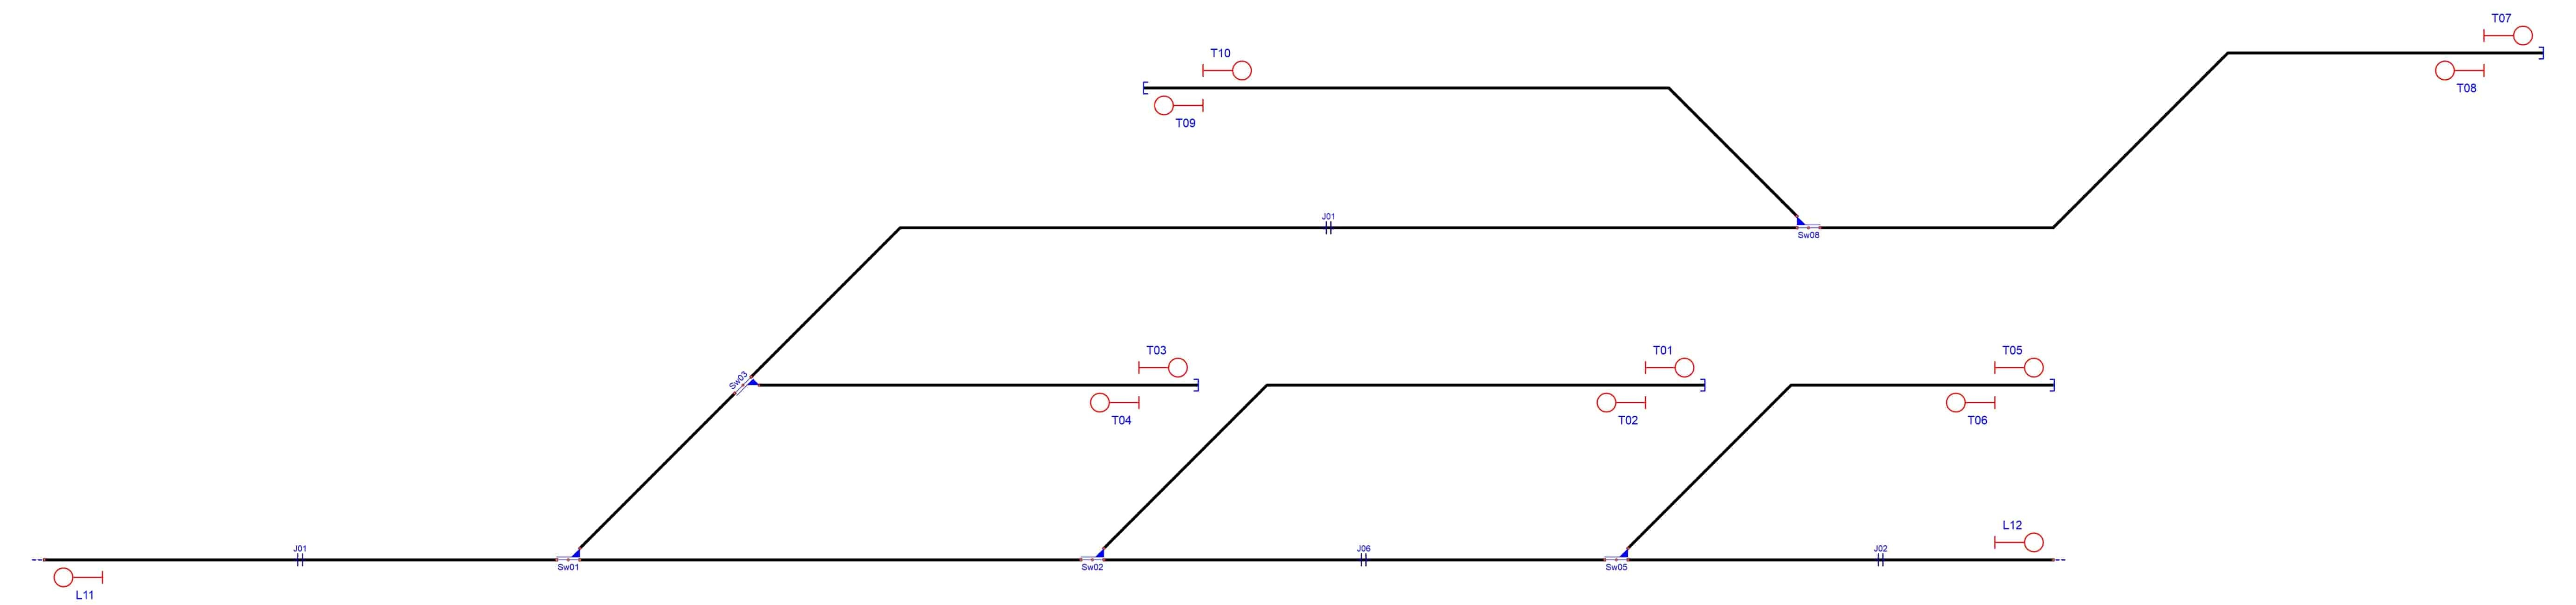
\includegraphics[width=1\textwidth]{resultados-obtenidos/ejemplo6/images/6_step1.png}
		\centering\caption{Señalamiento generado por el RNA para proteger el fín de vía.}
		\label{fig:EJ6_3}
	\end{figure}

	Los finales de vías absolutos son protegidos por las señales de parada T01, T03, T05, T07 y T09; y las señales de partida son T02, T04, T06, T08 y T10. A su vez, los finales de vías relativos poseen las señales de parada L11 y L12, cercanos al límite del externo del \textit{netElement} al que pertenecen.
	
	La Figura \ref{fig:EJ6_3} ilustra la generación de señales destinadas a proteger las junturas entre los rieles. Las señales generadas son todas las señales comprendidas entre J13 y J20, indicadas en color rojo.

	\begin{figure}[H]
		\centering
		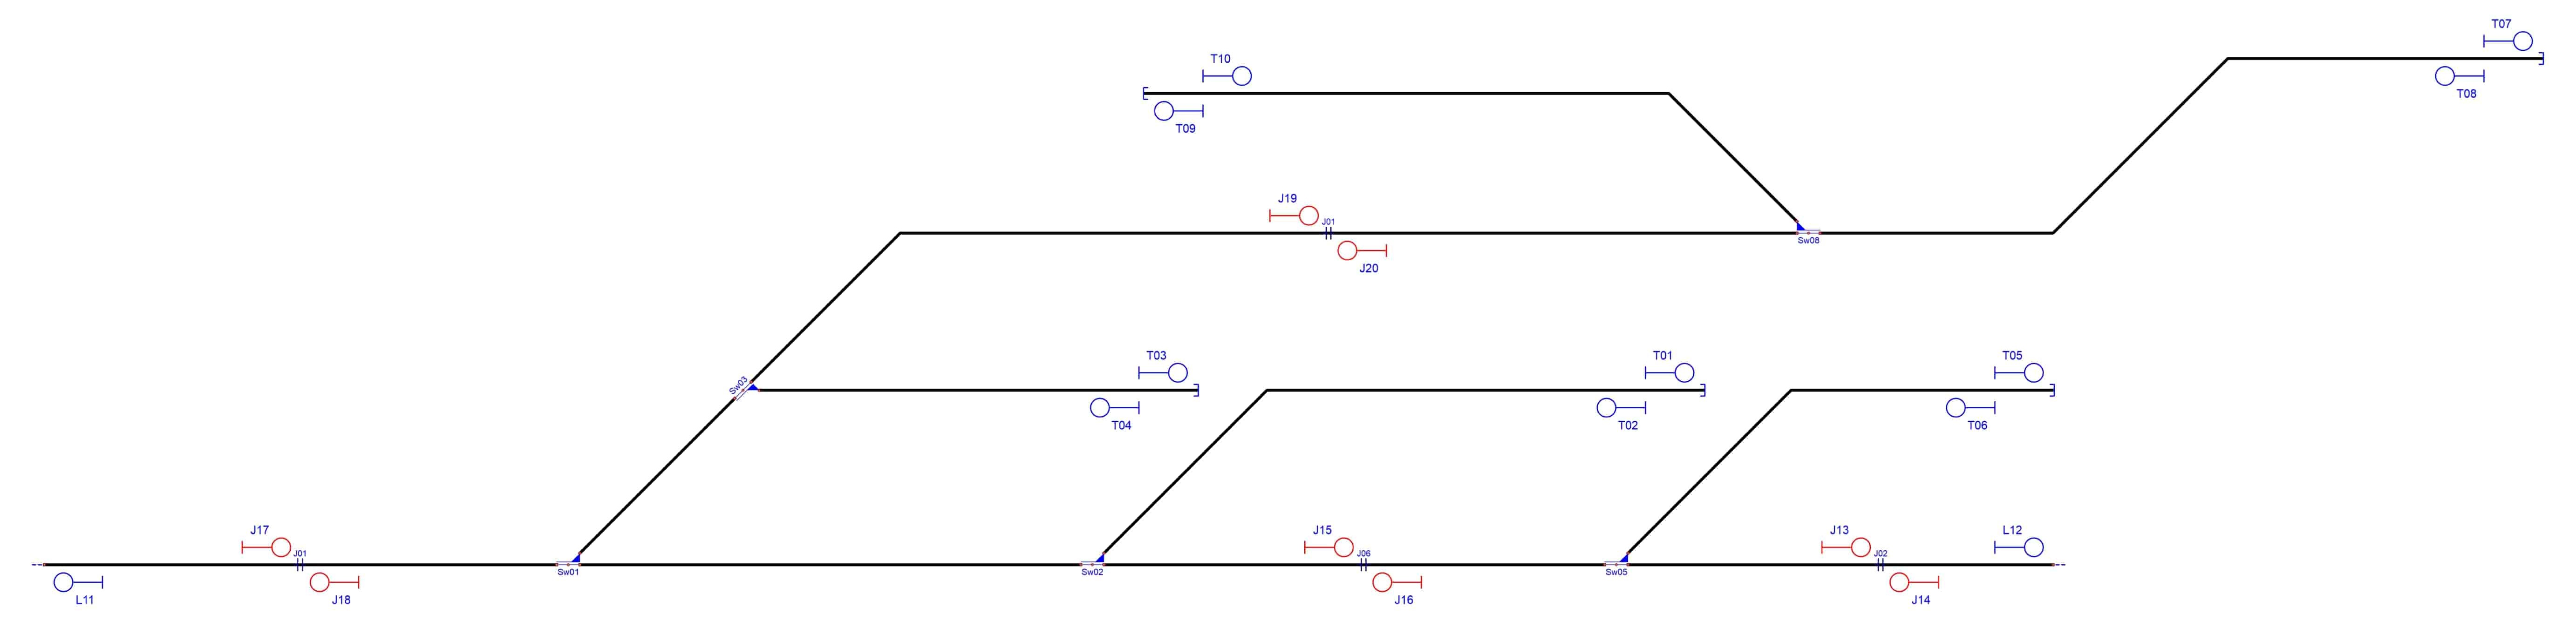
\includegraphics[width=1\textwidth]{resultados-obtenidos/ejemplo6/images/6_step2.png}
		\centering\caption{Señalamiento generado por el RNA para proteger las junturas.}
		\label{fig:EJ6_4}
	\end{figure}
	
	Al generar el señalamiento para proteger la infraestructura, tal como se explicó en la Sección \ref{sec:horizontal}, el Algoritmo \ref{alg:horizontal} simplificará las señales entre dos elementos ferroviarios si no existe espacio suficiente entre ellos. En este ejemplo, no existen plataformas o cruces de vías que proteger. Por lo tanto, el RNA no asigna nuevo señalamiento, como se visualiza en la Figura \ref{fig:EJ6_5}.

	\begin{figure}[H]
		\centering
		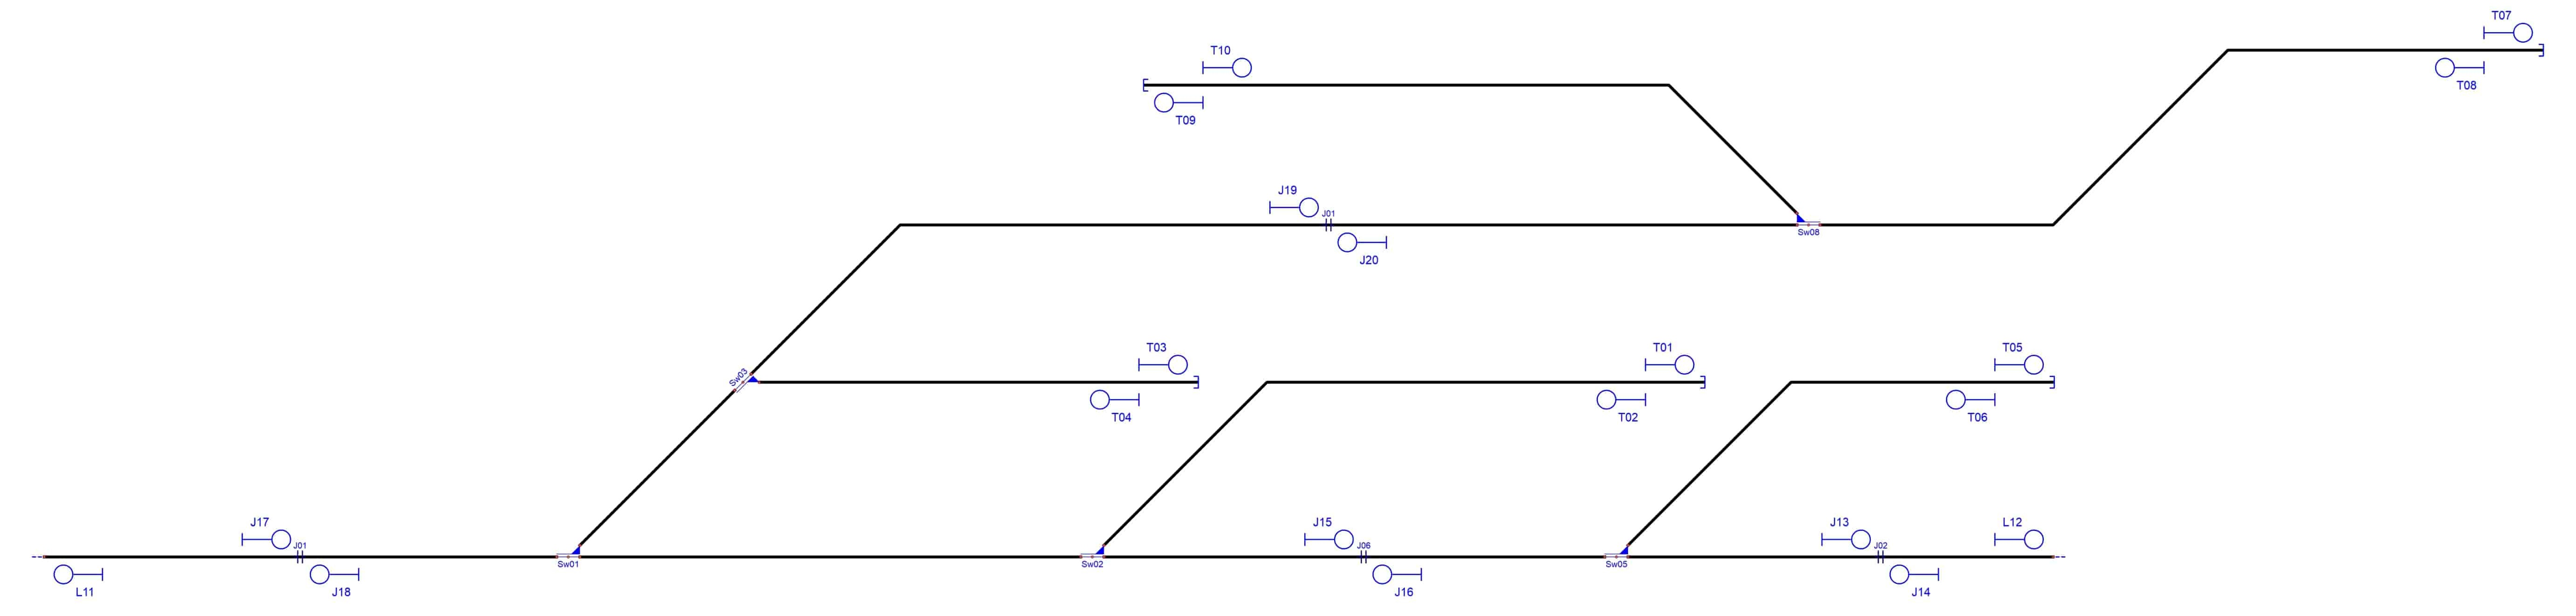
\includegraphics[width=1\textwidth]{resultados-obtenidos/ejemplo6/images/6_step3.png}
		\centering\caption{Señalamiento generado por el RNA para proteger plataformas y cruces de vía.}
		\label{fig:EJ6_5}
	\end{figure}

	El RNA generó las señales C21, S22 y H23 para proteger el cambio de vías Sw01; las señales C25, S27, B26 y H28 para proteger el cambio de vías Sw02; las señales C29, B30 Y H24 para proteger el cambio de vías Sw03; las señales C31, S33, B32 y H34 para proteger el cambio de vías Sw05 y las señales C35, S37, B36 y H38 para proteger el cambio de vías Sw08. Las señales mencionadas se encuentran resaltadas en rojo en la Figura \ref{fig:EJ6_6}.
	 \begin{figure}[H]
		\centering
		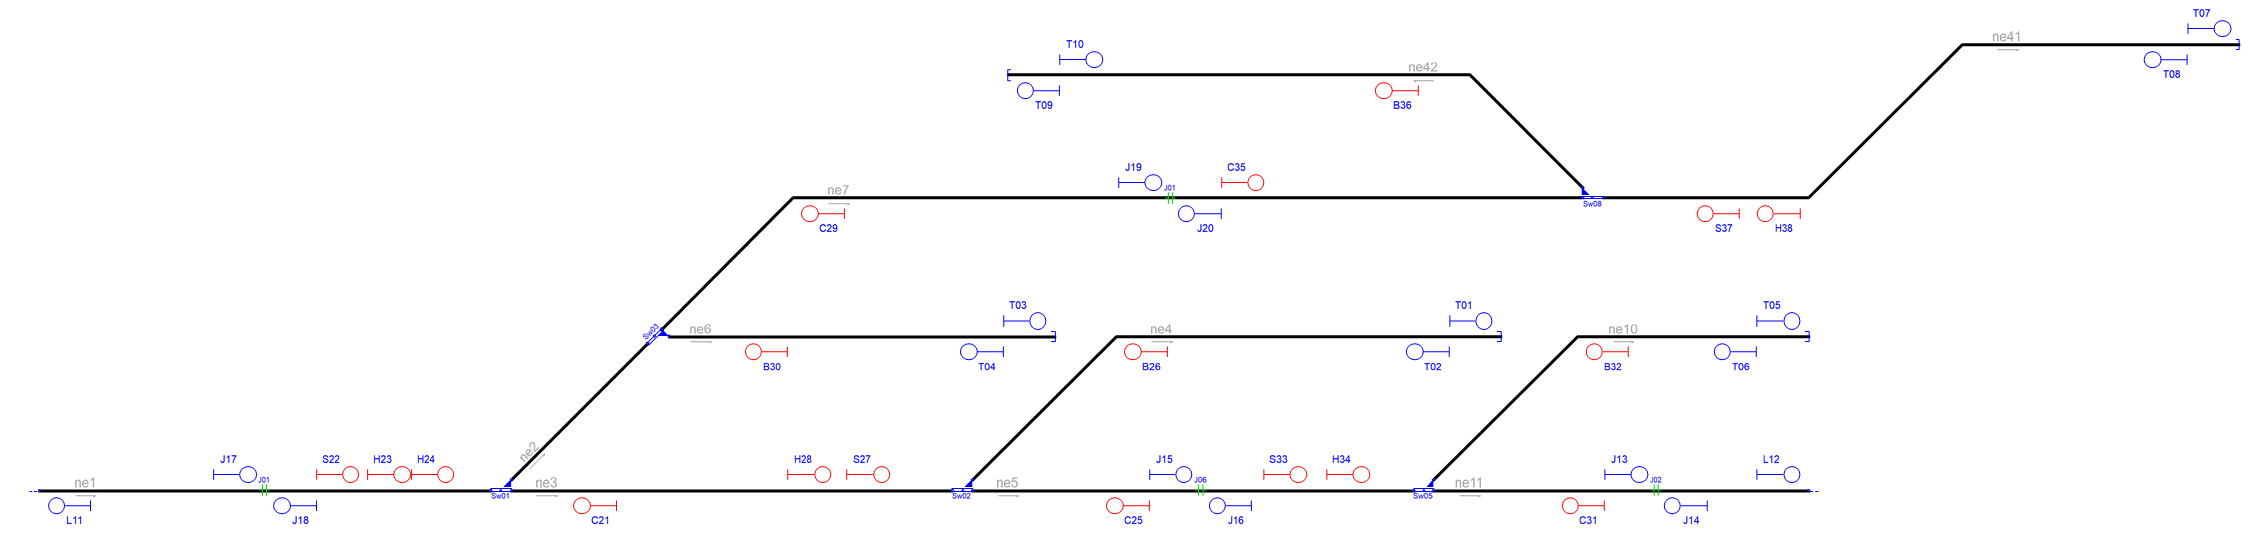
\includegraphics[width=1\textwidth]{resultados-obtenidos/ejemplo6/images/6_step4.png}
		\centering\caption{Señalamiento generado por el RNA para proteger las máquinas de cambios.}
		\label{fig:EJ6_6}
	\end{figure}
	
	Una vez obtenido todo el señalamiento, el RNA procede a simplificar las señales redundantes, repetidas o cuyas funciones o ubicaciones se superponen entre sí. El proceso de simplificación de señales fue explicado en la Sección \ref{sec:simplificacion}. El Algoritmo \ref{alg:vertical} de herencia vertical fue aplicado en la señal B del cambio de vías Sw01, moviéndola hasta la señal C29 del cambio de vías Sw03. Además, la señal S del cambio de vías Sw03 fue movida a la señal H23 del cambio de vías Sw01.
	
	Las señales simplificadas al aplicar el Algoritmo \ref{alg:horizontal} de herencia horizontal son: L12, J15, J17, H23, H24, C25, H28, B30, C31, B32, H34, C35 y H38. La señal H23 fue eliminada por su cercanía con la señal S22, con la cual comparten dirección y sentido. Lo mismo ocurre entre las señales H24 y S22; entre las señales H28 y S27; entre las señales H34 y S33; y entre las señales H38 y S37. En todos los casos, se aplicó el Algoritmo \ref{alg:horizontal}, diseñado para agrupar objetos cercanos como un único objeto, generando el señalamiento acorde a los elementos contenidos en cada extremo del nuevo elemento contenedor.
	
	Finalmente, las señales son simplificadas aplicando el Algoritmo \ref{alg:reduction} de eliminación por prioridad de señales. El resultado de este proceso es detallado en el Código \ref{lst:EJ6_3}.
	
	\begin{lstlisting}[language = {}, caption = Reducción de señalamiento por prioridad de señales, label = {lst:EJ6_3}]
	Reducing redundant signals
	T priority removing sig30 for sig04
	T priority removing sig32 for sig06
	L priority removing sig12 for sig13
	J>H priority removing sig31 for sig14
	J>S priority removing sig15 for sig33
	J>H priority removing sig25 for sig16
	J>S priority removing sig17 for sig22
	J>H priority removing sig35 for sig19
	Same position removing sig23 for sig22
	Same position removing sig24 for sig22
	Same position removing sig28 for sig27
	Same position removing sig34 for sig33
	Same position removing sig38 for sig37
	\end{lstlisting}

	El resultado de la simplificación del señalamiento se ilustra en la Figura \ref{fig:EJ6_7}.
	
	 \begin{figure}[H]
		\centering
		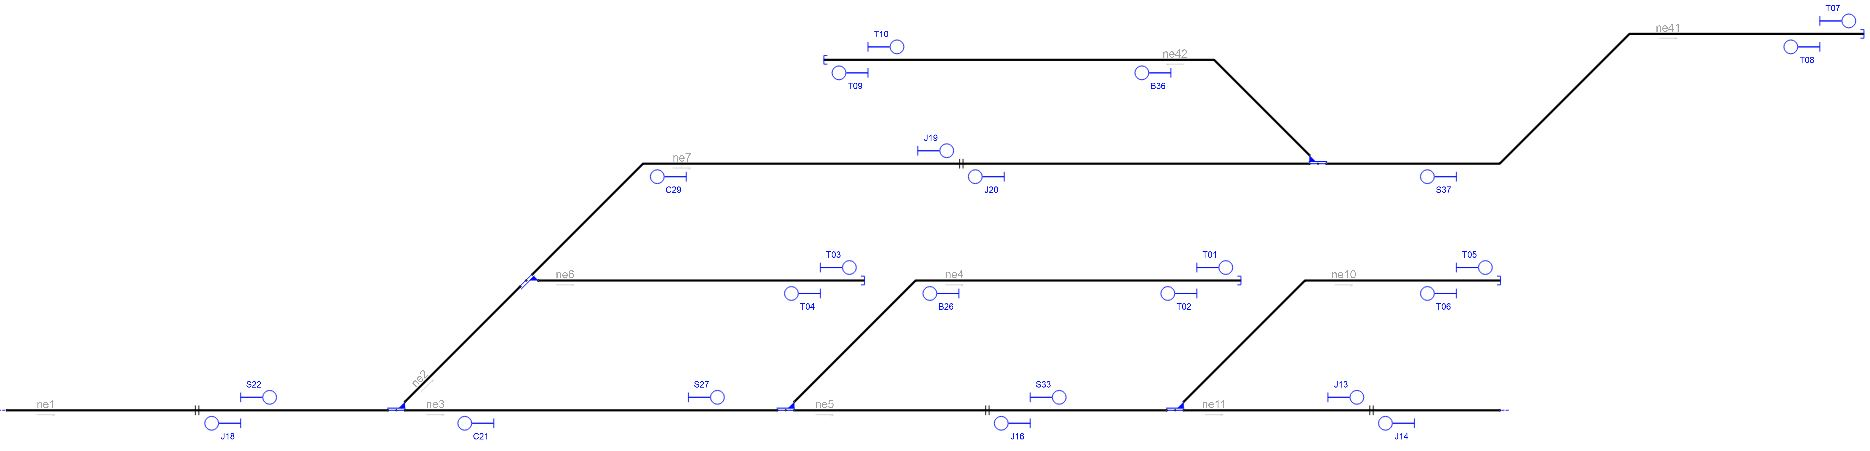
\includegraphics[width=1\textwidth]{resultados-obtenidos/ejemplo6/images/6_RNA.png}
		\centering\caption{Señalamiento generado y simplificado por el RNA.}
		\label{fig:EJ6_7}
	\end{figure}

	Al finalizar la generación del señalamiento, el RNA debe detectar todas las posibles rutas admitidas por la red para crear la tabla de enclavamientos. El RNA exporta los resultados del análisis en los siguientes cuatro documentos: Infrastructure.RNA (Apéndice \ref{sec:infrastructureRNA}), SafePoint.RNA (Apéndice \ref{sec:safePointsRNA}), Signalling.RNA (Apéndice \ref{sec:signallingRNA}) y Routes.RNA (Apéndice \ref{sec:routesRNA}).	